\documentclass[computergesteund_ontwerp_van_curven_en_oppervlakken.tex]{subfiles}
\begin{document}

\chapter{B\'ezier-curven}
\section{Bernstein-veeltermen}
\begin{de}
\label{bern}
De $i$-de \textbf{Bernstein-veelterm} van graad $n$ wordt als volgt gedefini\"eerd.
\[
B_{i}^{n} = \binom{n}{i}(1-t)^{n-i}t^{i}
\]
Defini\"eer bovendien $B_{i}^{n} = 0$ wanneer $i < 0$ of $i > n$ geldt.
\end{de}

\begin{ei} \textbf{\'E\'enheidspartitie}
\label{bern_eenheidspartitie}
\[
\sum_{i=0}^nB_{i}^{n}(t) = 1
\]
\begin{proof}
Gebruik eenvoudigweg het binomium van Newton.
\[
\sum_{i=0}^nB_{i}^{n}(t)
= \sum_{i=0}^{n}\binom{n}{i}(1-t)^{n-i}t^i
= ((1-t)+t)^n
= 1
\]
\end{proof}
\end{ei}

\begin{ei} \textbf{Positiviteit}
\label{bern_positiviteit}
\[
0 \le t \le 1 \Rightarrow B_{i}^{n}(t) \ge 0
\]
\begin{proof}
\[
\binom{n}{i}(1-t)^{n-i}t^{i}
\]
$\binom{n}{i}$ is positief, $(1-t)$ is positief want $0 \le t \le 1$ en $t$ is ook positief. De som van positieve getallen is steeds positief.
\end{proof}
\end{ei}


\begin{ei} \textbf{Randgevallen}
\begin{itemize}
\item $B_{i}^{n}(0) = B_{i}^{n}(1) = 0$ als $i\neq$, $i\neq n$.
\item $B_{0}^{n}(0) = 1$
\item $B_{0}^{n}(1) = 0$
\item $B_{n}^{n}(0) = 0$
\item $B_{n}^{n}(1) = 1$
\end{itemize}
\begin{proof}
Vul eenvoudigweg alles in.
\begin{itemize}
\item $B_{i}^{n}(0) = B_{i}^{n}\binom{n}{i}1^{n-i}0^{i} = 0$ en $B_{i}^{n}(1) = B_{i}^{n}\binom{n}{i}0^{n-i}1^{i} = 0$
\item $B_{0}^{n}(0) = 1^{n} = 1$
\item $B_{0}^{n}(1) = 0^{n} = 0$

\item $B_{n}^{n}(0) = 0^{n} = 0$
\item $B_{n}^{n}(1) = 1^{n} = 1$
\end{itemize}
\end{proof}
\end{ei}

\begin{ei}
\textbf{Symmetrie}
\[
B_{i}^{n}(t) = B_{n-i}^{n}(1-t)
\]
\begin{proof}
\[
\binom{n}{n-i}(1-1+t)^{n-n+i}(1-t)^{n-i}
= \binom{n}{i}t^{i}(1-t)^{n-i}
= \binom{n}{i}(1-t)^{n-i}t^{i} 
\]
\end{proof}
\begin{figure}[H]
\centering
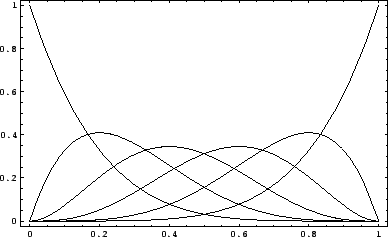
\includegraphics[scale=0.5]{illustraties/BernsteinPolynomial.png} 
\caption{Symmetrie van Bernstein-veeltermen voor $n=5$}
\end{figure}
\end{ei}

\begin{ei}
\textbf{Afgeleide}
\label{bern_afgeleide}
\[
\frac{d}{dt}B_{i}^{n}(t) = n(B_{i-1}^{n-1}(t) - B_{i}^{n-1}(t))
\]
\begin{proof}
\[
\frac{d}{dt}B_{i}^{n}(t) = \frac{d}{dt}\binom{n}{i}(1-t)^{n-i}t^{i}
\]
\[
\binom{n}{i}\frac{d}{dt}\left((1-t)^{n-i}t^{i}\right)
= \binom{n}{i}
\left(
t^{i}\frac{d}{dt}(1-t)^{n-i}
+ (1-t)^{n-i}\frac{d}{dt}t^{i}
\right)
\]
\[
\binom{n}{i}\frac{d}{dt}\left((1-t)^{n-i}t^{i}\right)
= \binom{n}{i}
\left(
(1-t)^{n-i}it^{i-1}
-t^{i}(n-i)(1-t)^{n-i-1}
\right)
\]
\[
= 
\left(
\frac{n!}{i!(n-i)!}
(1-t)^{n-i}it^{i-1}
-
\frac{n!}{i!(n-i)!}
t^{i}(n-i)(1-t)^{n-i-1}
\right)
\]
\[
= 
n
\left(
\frac{(n-1)!}{(i-1)!(n-i)!}
(1-t)^{n-i}t^{i-1}
-
\frac{(n-1)!}{i!(n-i-1)!}
t^{i}(1-t)^{n-i-1}
\right)
\]
\[
 = n(B_{i-1}^{n-1}(t) - B_{i}^{n-1}(t))
\]
\end{proof}
\end{ei}
\begin{ei}
Extrema
\[
\frac{d}{dt}B_{i}^{n}(t) = 0 \Leftrightarrow t = \frac{i}{n} \text{ voor } n > 0 \text{ en } 0 < i < n
\]
\begin{proof}
\[
\frac{d}{dt}B_{i}^{n}(t) = n(B_{i-1}^{n-1}(t) - B_{i}^{n-1}(t)) = 0
\]
\[
nB_{i-1}^{n-1}(t) = nB_{i}^{n-1}(t)
\]
\[
n \frac{(n-1)!}{(i-1)!(n-i)!}
(1-t)^{n-i}t^{i-1}
=
n \frac{(n-1)!}{i!(n-i-1)!}
(1-t)^{n-i-1}t^{i}
\]
\[
\frac{(1-t)}{n-i}
=
\frac{t}{i}
\]
\[
t = \frac{i}{n}
\]
\end{proof}
\end{ei}
\begin{ei}
Recursiebetrekking.
\[
B_{i}^{n}(t) = (1-t)B^{n-1}_{i}(t) + tB^{n-1}_{i-1}(t)
\]
\begin{proof}
\[
(1-t)B^{n-1}_{i}(t) + tB^{n-1}_{i-1}(t)
\]
\[
= 
(1-t)\binom{n-1}{i}
(1-t)^{n-i-1}t^{i}
+
t\binom{n-1}{i-1}
(1-t)^{n-i}t^{i-1} 
\]
\[
= \left(\binom{n-1}{i}+\binom{n-1}{i-1}\right)
(1-t)^{n-i}t^{i}
\]
\[
=
\binom{n}{i}
(1-t)^{n-i}t^{i}
= B_{i}^{n}(t)
\]
\end{proof}
\end{ei}

\section{B\'ezier curve}
\begin{de}
Een B\'ezier curve met $n+1$ controlepunten is een lineaire combinatie van de controlepunten met Bernstein-veeltermen als gewichten.
\[
x(t) = \sum_{i=0}^nb_{i}B_{i}^{n}(t)
\]
\end{de}

\begin{ei}
\label{bezier_veelterm}
Een B\'ezier-curve is een veeltermcurve van graad $n$.
\begin{proof}
\[ng voor bernstein-veeltermen.
\sum_{i=0}^nb_{i}B_{i}^{n}(t) = \sum_{i=0}^nb_i\frac{n!}{i!(n-i)!}(1-t)^{n-i}t^{i}
\]
De hoogste graad van $t$ komt voor wanneer $i$ nul is. Dan is die graad $n$.
\end{proof}
\end{ei}

\begin{ei}
$x(t)$ is een affiene combinatie van de controlepunten $b_i$. $x(t)$ is dus een punt dat afhangt van de parameter $t$.
\begin{proof}
De som van alle $B_{i}^{n}(t)$ is $1$.\footnote{Zie eigenschap \ref{bern_eenheidspartitie} van Bernstein-veeltermen.} Dit geldt voor elke $t$.
\end{proof}
\end{ei}

\begin{ei}
Het verband tussen de B\'ezier curve en de B\'ezier punten is invariant onder affiene transformaties.
\begin{proof}
Zij $L$ een affiene transformatie.
\[
L(x(t))
= L\left( \sum_{i=0}^nb_{i}B_{i}^{n}(t)\right)
= \sum_{i=0}^nL(b_{i})B_{i}^{n}(t)
\]
\end{proof}
\end{ei}

\begin{ei}
Elk punt op een B\'ezier curve light binnen de convex omhullende van de controlepunten.
\begin{proof}
Elk punt van de Bezier-curve is een convexe combinatie van de controle punten want elke Bernstein-veelterm is positief. \footnote{Zie eigenschap \ref{bern_positiviteit} van Berstein-veeltermen.} Omdat elk punt op de curve een convexe combinatie is, ligt elk punt binnen de convex omhullende van de controlepunten. \footnote{Zie stelling \ref{combinatie_in_omhullende}.}
\end{proof}
\end{ei}

\begin{ei}
De B\'ezier curve interpoleert in het eerste en laatste controlepunt.
\begin{proof}
In $t=0$ interpoleert de B\'ezier curve in het eerste controlepunt. In $t=1$ interpoleert de B\'ezier curve in het laatste controlepunt.
\begin{itemize}
\item
\[
x(0) = \sum_{i=0}^nb_{i}B_{i}^{n}(0) = B_{0}^nb_0 = b_0
\]

\item
\[
x(1) = \sum_{i=0}^nb_{i}B_{i}^{n}(1) = B_{n}^nb_n = b_n
\]
\end{itemize}
\end{proof}
\end{ei}

\begin{ei}
Variatie-verminderingseigenschap\\
Het aantal snijpunten van een willekeurige rechte (in 2D) of vlak (in 3D) met de B\'ezier-curve is kleiner dan of gelijk aan het aantal snijpunten van die rechte (of vlak) met de Controleveelhoek. In mensentaal: de curve zal minder ``wiebelen'' dan de controleveelhoek.
\end{ei}

\subsection{Evaluatie van een punt op een B\'ezier curve (de Castejau)}
\begin{st}
Zij $b_{i}^{[0]} = b_{i}$ en definieer $b_{i}^{[k]}$ recursief als volgt.
\[
b_{i}^{[k]}
=
(1-t)b_{i-1}^{[k-1]} + tb_{i}^{[k-1]}
\]
Nu geldt volgende bewering.
\[
x = b_{n}^{[n]} = \sum_{i=0}^{n}b_iB_{i}^{n}(t)
\]
De B\'ezier curve kan dus recursief berekend worden.
\begin{proof}
\[
x(t) = \sum_{i=0}^{n}b_iB_{i}^{n}(t)
\]
Gebruik de recursiebetrekking voor bernstein-veeltermen.
\[
= \sum_{i=0}^{n}b_i
\left( 
(1-t)B^{n-1}_{i}(t) + tB^{n-1}_{i-1}(t)
\right)
= 
\sum_{i=0}^{n}b_i
(1-t)B^{n-1}_{i}(t) + 
\sum_{i=0}^{n}b_it
B^{n-1}_{i-1}(t)
\]
De eerste en laatste term van deze uitdrukking kunnen we weglaten ($B_{i}^{n} = 0$ als $i < 0$ of $i > n$ \footnote{Zie definitie \ref{bern}}).
\[
= 
\sum_{i=0}^{n-1}b_i
(1-t)B^{n-1}_{i}(t) + 
\sum_{i=1}^{n}b_it
B^{n-1}_{i-1}(t)
\]
Merk op dat alle $b_i$ gelijk zijn aan $b_i^{[0]}$. We proberen ze nu zo te schrijven dat we er $b_i^{[1]}$ van kunnen maken. Vervang de $i$ in de eerste term door $j=i+1$ en hernoem daarna $j$ naar $i$. In feite schuiven we de sommatie-index $1$ \'e\'enheid op.
\[
= 
\sum_{i=1}^{n}b_{i-1}
(1-t)B^{n-1}_{i-1}(t) + 
\sum_{i=1}^{n}b_it
B^{n-1}_{i-1}(t)
\]
Nu zien we dat de sommaties dezelfde zijn. We kunnen deze dus buiten brengen omdat de optelling commutatief is.
\[
= 
\sum_{i=1}^{n}
\left(
b_{i-1}(1-t)B^{n-1}_{i-1}(t)
+ 
b_itB^{n-1}_{i-1}(t)
\right)
\]
\[
= 
\sum_{i=1}^{n}
B^{n-1}_{i-1}(t)
\left(
(1-t)b_{i-1}
+ 
tb_i
\right)
\]
Kijk nu naar de zojuist gedefini\"eerde recursiebetrekking. We kunnen $(1-t)b_{i-1} + tb_i = (1-t)b_{i-1}^{[0]} + tb_i^{[0]}$ vervangen door $b_{i}^{[1]}$
\[
= 
\sum_{i=1}^{n}
B^{n-1}_{i-1}(t)
b_{i}^{[1]}
\]
Als we dit proces nog eens herhalen krijgen we de volgende uitdrukking.
\[
= 
\sum_{i=2}^{n}
B^{n-2}_{i-2}(t)
b_{i}^{[2]}
\]
In de $j$-de iteratie ziet het nieuwe rechterlid er als volgt uit.
\[
= 
\sum_{i=j}^{n}
B^{n-j}_{i-j}(t)
b_{i}^{[j]}
\]
Dit proces kunnen we $n$ (eindig en zelfs een lineair aantal) keer uitvoeren tot we volgende uitdrukking bekomen.
\[
\sum_{i=n}^{n}
B^{0}_{0}(t)
b_{i}^{[n]}
= b_{n}^{[n]}
\]
\end{proof}
\end{st}
Deze bewering geeft een algoritme om een punt op de B\'ezier-curve recursief te berekenen. De index in superscript tussen vierkante haakjes heeft betrekking tot de iteratie waarin dit punt zich bevindt. In de praktijk wordt het principe van ``dynamic'' programming ingezet, zodat het algoritme een complexiteit heeft van $O(n^2)$ in plaats van $O(2^n)$.

\subsection{Afgeleide van een B\'ezier-curve}
\begin{st}
\[
\frac{d}{dt}x(t) = n\sum_{i=0}^{n-1}\Delta b_iB_{i}^{n-1}(t)
\]

\begin{proof}
\[
\frac{d}{dt}x(t)
= \frac{d}{dt}\sum_{i=0}^{n}b_iB_{i}^{n}(t)
= \sum_{i=0}^{n}b_i\frac{d}{dt}B_{i}^{n}(t)
\]
Gebruik de uitdrukking voor de afgeleide van een Bernstein veelterm.\footnote{Zie eigenschap \ref{bern_afgeleide} van Bernstein veeltermen.}
\[
= \sum_{i=0}^{n}b_i n(B_{i-1}^{n-1}(t) - B_{i}^{n-1}(t))
= n\sum_{i=0}^{n}b_i (B_{i-1}^{n-1}(t) - B_{i}^{n-1}(t))
\]
Splits de sommatie.
\[
= n\sum_{i=0}^{n}b_i B_{i-1}^{n-1}(t)
- n\sum_{i=0}^{n}b_i B_{i}^{n-1}(t)
\]
De eerste en de laatste term in deze uitdrukking zijn beide nul.\footnote{Zie definitie \ref{bern}.}
\[
= n\sum_{i=1}^{n}b_i B_{i-1}^{n-1}(t)
- n\sum_{i=0}^{n-1}b_i B_{i}^{n-1}(t)
\]
Schuif het linkse sommatie teken \'e\'en index op.
\[
= n\sum_{i=0}^{n-1}b_{i+1} B_{i}^{n-1}(t)
- n\sum_{i=0}^{n-1}b_i B_{i}^{n-1}(t)
\]
\[
= n\sum_{i=0}^{n-1}(b_{i+1}-b_i)B_{i}^{n-1}(t) 
\]
\[
= n\sum_{i=0}^{n-1}\Delta b_iB_{i}^{n-1}(t)
\]
\end{proof}
\end{st}

\subsection{Interpolatie in de eindpunten}
\begin{ei}\textbf{Interpolatie in de eindpunten}\\
Een B\'ezier curve raakt in het eerste en laatste controlepunt (waar die interpoleert) aan de controleveelhoek.
\[
\left.\frac{d}{dt} x(t)\right|_{t=0} = a(b_1-b_{0})
\text{ en }
\left.\frac{d}{dt}x(t)\right|_{t=1} = b(b_n-b_{n-1})
\]
\[
\]
of voor meervoudige B\'ezier curven:
\[
\left.\frac{d}{du}x(t(u))\right|_{t=0} = a'(b_1-b_{0})
\text{ en }
\left.\frac{d}{du}x(t(u))\right|_{t=1} = b'(b_n-b_{n-1})
\]
($a$, $a'$, $b$, $b'$ zijn hier bepaalde scalars.) 

\begin{proof}
We bewijzen elk deel appart.
\begin{itemize}
\item
\begin{itemize}
\item
\[
\frac{d}{dt}x(t)|_{t=0}
= \left.n\sum_{i=0}^{n-1}\Delta b_iB_{i}^{n-1}(t)\right|_{t=0}
\]
\[
= \sum_{i=0}^{n-1}\Delta b_iB_{i}^{n-1}(0)
= n\Delta b_0
\]
\item
\[
\left.\frac{d}{dt}x(t)\right|_{t=1}
= \left.n\sum_{i=0}^{n-1}\Delta b_iB_{i}^{n-1}(t)\right|_{t=1}
\]
\[
= \sum_{i=0}^{n-1}\Delta b_iB_{i}^{n-1}(1)
= n\Delta b_{n-1}
\]
\end{itemize}
\item
\begin{itemize}
\item
\[
\left.\frac{d}{du}x(t(u))\right|_{t=0} = a'(b_1-b_{0})
\]
\[
\frac{n}{\Delta u}\sum_{i=0}^{n-1}\Delta b_iB_{i}^{n-1}(0)
= \frac{n}{\Delta u}\Delta b_{0}
\]
\item
\[
\left.\frac{d}{du}x(t(u))\right|_{t=1} = b'(b_n-b_{n-1})
\]
\[
\frac{n}{\Delta u}\sum_{i=0}^{n-1}\Delta b_iB_{i}^{n-1}(1)
= \frac{n}{\Delta u}\Delta b_{n-1}
\]
\end{itemize}
\end{itemize}
\end{proof}
\end{ei}





\subsection{Hogere afgeleiden}
Tweede afgeleide:
\[
\frac{d^2}{dt}x(t) = n(n-1) \sum_{i=0}^{n-2}\Delta^2b_iB_{i}^{n-2}(t)
\]
$j$-de afgeleide:
\[
\frac{d^j}{dt}x(t) = \frac{n!}{(n-j)!}\sum_{i=0}^{n-j}\Delta^{j}b_iB_{i}^{n-j}(t)
\]

\section{Graadverhoging}
Elke veelterm van graad $n$ kan geschreven worden als een veelterm van graad $n+1$. Er moet dus ook een manier zijn om een B\'eziercurve van graad $n$ te schrijven als een B\'eziercurve van graad $n+1$.\footnote{Inderdaad! Zie eigenschap \ref{bezier_veelterm} van B\'eziercurven.} 
\[
\sum_{i=0}^{n}b_iB_{i}^{n}(t) = \sum_{i=0}^{n+1}b_i^*B_{i}^{n+1}(t)
\]
\begin{st}
De nieuwe controlepunten $b_i^*$ kunnen berekend worden uit de originele controlepunten.
\[
b^*_i= \frac{i}{n+1}b_{i-1} + \left(1-\frac{1}{n+1}\right)b_i
\]
\begin{proof}
Let op: niet vanzelfsprekend.
\[
x(t)
= \sum_{i=0}^{n}b_i\binom{n}{i}(1-t)^{n-i}t^{i}
= \left(\sum_{i=0}^{n}b_i\binom{n}{i}(1-t)^{n-i}t^{i}\right) (t+(1-t))
\]
\[
= \left(\sum_{i=0}^{n}b_i\binom{n}{i}(1-t)^{n-i}t^{i+1}\right)
+ \left(\sum_{i=0}^{n}b_i\binom{n}{i}(1-t)^{n-i+1}t^{i}\right)
\]
Verander de index van de eerste term.
\[
= \left(\sum_{i=1}^{n+1}b_{i-1}\binom{n}{i-1}(1-t)^{n-i+1}t^{i}\right)
+ \left(\sum_{i=0}^{n}b_i\binom{n}{i}(1-t)^{n-i+1}t^{i}\right)
\]
Neem beide sommaties samen. Dit kan omdat we $\binom{n}{-1}$ en $\binom{n}{n+1}$ als nul defini\"eren.
\[
= \sum_{i=0}^{n+1}(1-t)^{n-i+1}t^{i} \left(\binom{n}{i-1}b_{i-1} + \binom{n}{i}b_i\right)
\]
We halen hier de nieuwe controlepunten uit.
\[
\binom{n+1}{i}b_{i}^{*}
= \binom{n}{i-1}b_{i-1}
+ \binom{n}{i}b_i
\]
\[
\frac{(n+1)!}{i!(n-i+1)!}b_{i}^{*}
= \frac{n!}{(i-1)!(n-i+1)!} b_{i-1}
+ \frac{n!}{i!(n-i)!}b_i
\]
\[
b_{i}^{*}
= \frac{i}{n+1} b_{i-1}
+ \left(1-\frac{1}{n+1}\right)b_i
\]
\end{proof}
\end{st}

\section{Opsplitsing}
Gegeven een B\'ezier curve van graad $n$, willen we deze opsplitsen in twee nieuwe curven van graad $n$ met elk $n+1$ controlepunten $d_i$ en $e_i$ respectievelijk. Zij $t$ de parameter voor de originele curve met $t \in [0,1]$. Noem $c$ het punt in het parameter interval van $t$ waar we de curve splitsen. We krijgen dan twee curven met parameter $s$ en $r$, respectievelijk . $s$ en $r$ zitten dan in de intervallen $[0,c]$ en $[c,1]$ respectievelijk.
Gegeven $t$ kunnen we nu $s$ en $r$ bepalen.
\[
\left\{
\begin{array}{c l}
s(t) &= \frac{t}{c}\\
r(t) &= c + \frac{(1-t)}{c}\\
\end{array}
\right.
\]
We zoeken nu de nieuwe controlepunten $d_i$ en $e_i$ voor de twee nieuwe curven. $v(s(t))$ en $w(r(t))$ zien er dan als volgt uit.
\[
\left\{
\begin{array}{c c}
v(s(t)) &= \sum_{i=0}^{n}d_iB^{n}_{i}(s)\\
w(r(t)) &= \sum_{i=0}^{n}e_iB^{n}_{i}(r)
\end{array}
\right.
\]
\begin{st}
We kunnen de $d_i$ en $e_i$ eenvoudig berekenen uit het algoritme van de Casteljau voor evaluatie van $x(c)$ als volgt.
\[
\forall i: d_i = b_{i}^{[i]}\ \text{ en }\ \forall i: e_i = b_{n-i}^{[n-i]}
\]
\begin{proof}
Vermist $v(s(t))$ (en $w(r(t))$) deel uitmaken van dezelfde unieke veeltermcurve van graad $n$, zijn alle afgeleiden van $v(s(t))$ en $x(t)$ naar $t$ aan elkaar gelijk in $t=0$. Bovendien zijn alle afgeleiden van $w(r(t))$ en $x(t)$ naar $t$ gelijk aan elkaar in $t=1$.
\[
k = 0,\cdots,n:\
\left.\ \frac{d^{k}}{dt^{k}}v(s(t))\ \right|_{t=0} = \left.\  \frac{d^{k}}{dt^{k}}x(t)\ \right|_{t=0} 
\] 
\[
k = 0,\cdots,n:\
\left.\ \frac{d^{k}}{dt^{k}}w(r(t))\ \right|_{t=1} = \left.\  \frac{d^{k}}{dt^{k}}x(t)\ \right|_{t=1} 
\] 

\begin{itemize}
\item $k=0$:
\[
d_0 = b_0 =b_0^{[0]} \text{ en } e_n = b_n = b_{n}^{n}
\]

\item $k=1$:
\[
\frac{d}{dt}v(s(0)) = \frac{d}{dt}x(0) \text{ en } \frac{d}{dt}w(r(1)) = \frac{d}{dt}x(1)
\]
\begin{itemize}
\item
\[
\frac{ds}{dt}n\Delta d_0 = n\Delta b_0
\]
\[
\frac{n}{c}(d_1-d_0) = n(b_1-b_0)
\]
\[
\frac{1}{c}(d_1-b_0) = b_1-b_0
\]
\[
d_1 = (1-c)b_0+cb_1 = b_1^{[1]}
\]

\item
\[
\frac{dr}{dt}n\Delta d_{n-1} = n\Delta b_{n-1}
\]
\[
-\frac{n}{c}(e_n-e_{n-1}) = n(b_{n}-b_{n-1})
\]
\[
-\frac{1}{c}(b_{n}-e_{n-1}) = b_{n} - b_{n-1}
\]
\[
e_{n-1} = (c-1)b_{n} - b_{n-1} = b_{n-1}^{n-1}
\]

\end{itemize}

\item $k=j$:
\begin{itemize}
\item
\[
\frac{d^{j}}{dt^{j}}v(s(0)) = \frac{d^{j}}{dt^{j}}x(0)
\]
\[
\frac{d^{j}s}{dt^{j}}\frac{n!}{c^j(n-j)!}\Delta^{j}d_i
= \frac{n!}{(n-j)!}\Delta^{j}b_i
\]
\[
d_{j} = \sum_{i=0}^j{j \choose i}(1-c)^{j-i}c^ib_i= b_j^{[j]}
\]

\item
\[
\frac{d^{j}}{dt^{j}}w(r(1)) = \frac{d^{j}}{dt^{j}}x(1)
\]
\[
\frac{d^{j}r}{dt^{j}}\frac{n!}{c^j(n-j)!}\Delta^{j}e_i
= \frac{n!}{(n-j)!}\Delta^{j}b_i
\]
\[
e_{j} = -\sum_{i=0}^j{j \choose i}(c-1)^{j-i}c^ib_k= b_{n-j}^{[n-j]}
\]
\end{itemize}
\end{itemize}
\end{proof}
\end{st}
\section{Samengestelde Be\'ezier-curven}
Een samengestelde B\'ezier-curve over een parameterinterval $[u_0,u_p]$ is een stuksgewijze veeltermcurve, waarbij ieder segment een B\'ezier-curve is, gedefinieerd over \'e\'en van de intervallen $[u_0,u_1],[u_1,u_2],\cdots,[u_{p-1},u_{p}]$, bepaald door de knooppunten $u_0<u_1<u_2<\cdots u_p$
\[
x(u) = x_i(t(u))
\]
De samengestelde B\'ezier-curve bestaat dus uit $p$ segmenten $x_i(t(u))$ die elk veeltermcurven zijn. Elk segment $x_i$ wordt bepaald door haar eigen parameterinterval $[u_i,u_{i+1}]$ en heeft zodoende een locale parameter $t$.
\[
t = \frac{u-u_i}{u_{i+1}-u_i}
\]

\subsection{Afgeleide van meervoudige B\'ezier-curve}
\begin{ei}
Zij $t$ in het segment $[u_i,u_{i+1}]$:
\[
\frac{d}{du}x(t(u))
= \frac{n}{\Delta u}\sum_{i=0}^{n-1}\Delta b_iB_{i}^{n-1}(t)
\]
\begin{proof}
\[
t = \frac{u-u_i}{u_{i+1}-u} \text{ zodat } \frac{dt}{du} = \frac{1}{u_{i+1}-u}
\]
\[
\frac{d}{du}x(t(u))
= \frac{d}{dt} x(t) \frac{dt}{du}
= \frac{n}{u_{i+1}-u_i}\sum_{i=0}^{n-1}\Delta b_iB_{i}^{n-1}(t)
\]
\[
= \frac{n}{\Delta u_i}\sum_{i=0}^{n-1}\Delta b_iB_{i}^{n-1}(t)
\]
\end{proof}
\end{ei}

\subsection{Continu\"iteit}
We willen de afzonderlijke B\'ezier-curven laten aansluiten op een continu\"e manier.

Om deze sectie eenvoudig te houden gebruiken we telkens een voorbeeld van de samenstelling van twee kubische spline curves.

\subsubsection{$C^{0}$ continu\"iteit}
$C^{0}$ continu\"iteit verkrijgen we wanneer het laatste punt van de eerste curve gelijk is aan het eerste punt van de tweede curve.
\[
b_3 = b_0^*
\]
De opeenvolgende segmenten hebben dus de eindpunten gemeen.

\subsubsection{$C^{1}$ continu\"iteit}
$C^{1}$ continu\"iteit verkrijgen we als de rechte door de laatste twee punten van de eerste curve gelijk is aan de rechte door de eerste twee punten van de tweede curve.
\[
\frac{3}{u_1-u_0}(b_3-b_2) = \frac{3}{u_2-u_1}(b_1^{*}-b_0^{*})
\]

\subsubsection{$G^{1}$ continu\"iteit}
Eerste orde geometrische continu\"iteit verkrijgen we als de drie punten op de scheiding collineair zijn. De verhoudingen van de onderlinge afstanden spelen dan geen rol.

\subsubsection{$C^{2}$ continu\"iteit}
$C_{2}$ continu\"iteit verkrijgen we als de samengestelde curve $C^{1}$-continu is en ook de tweede afgeleiden gelijk zijn in het knooppunt.
\[
\frac{6}{(u_1-u_0)^2}(b_3-2b_2+b_1)
= \frac{6}{(u_1-u_0)^2}(b_2^*-2b_1^*+b_0^*)
\]


\end{document}
